\section{系统设计}

\subsection{需求分析与模块选型}

根据一般企事业单位对于考勤事务的管理规范,本指纹考勤系统需要实现以下几种功能,通过上位机对于下位机中指纹识别模块保存的指纹信息进行注册与删除,下位机基于前者提供的指纹数据实现基于光学识别的指纹打开签到功能。

根据上述系统功能需求,本设计以树莓派 4B 嵌入式开发板所提供的 bcm2711 作为中央处理芯片
,指纹考勤系统主要由电源供电模块,声音反馈模块,USB转TTL串口通信模块,网卡模块。
系统总体设计方案如\ref{总体设计图}所示。

% https://www.processon.com/v/65ec0156778cc21034664557
\begin{figure}[ht]
    \centering
    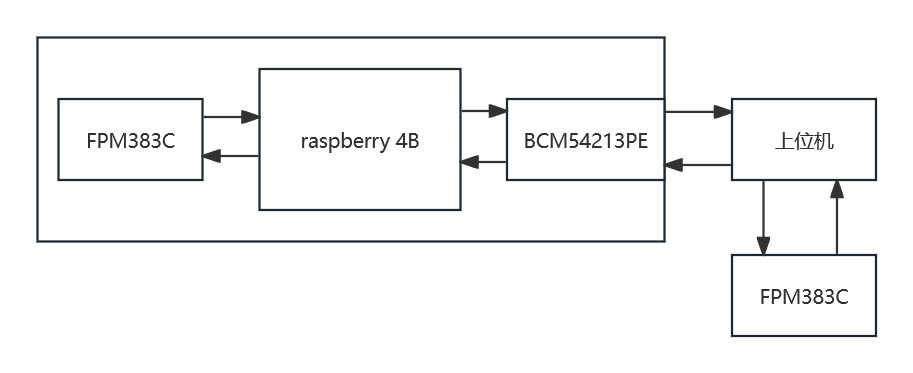
\includegraphics[width=\textwidth]{imgs/总体设计图.png}
    \caption{总体设计图}    \label{总体设计图}
\end{figure}

\subsubsection{嵌入式开发板选型}

树莓派 4B \ref{树莓派硬件配置说明图}使用的 bcm2711 是一颗四核心 64 位 ARM Cortex-A72 架构 CPU ,主频高,能满足多种复杂计算需求以及满足大型程序运行需求。
树莓派 4B 还存在丰富而完善的接口,两个 USB3.0 接口、两个 USB2.0 接口、一个千兆网卡接口、一个 HDMI 接口、一个 CSI 接口和一个 DSI 接口,能够满足对于各种外设的连接需求。
树莓派 4B 还是首款支持不通过 USB 接口而直接访问网卡芯片以实现网络连接的树莓派开发板,
这无形之中对于实现板载网卡驱动提供了很多帮助。

\begin{figure}[ht]
    \centering
    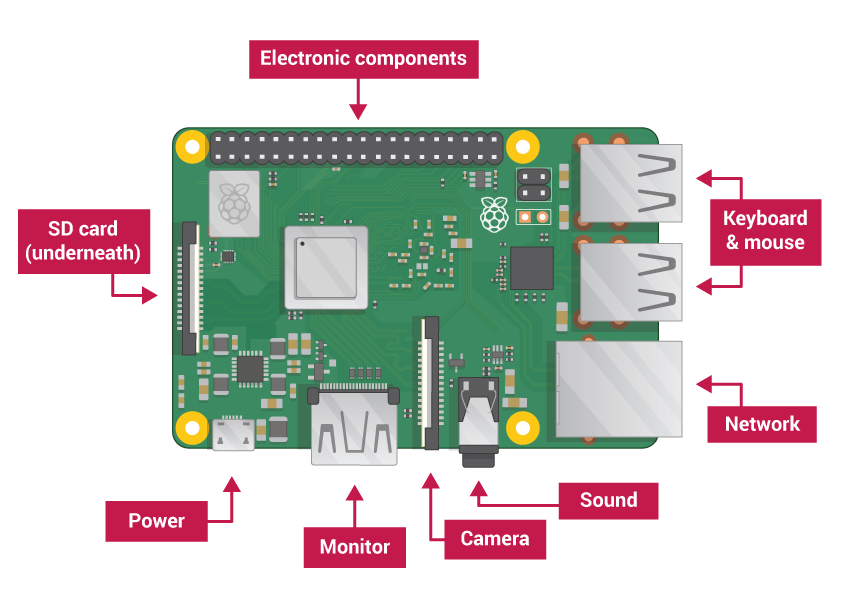
\includegraphics[width=\textwidth]{imgs/树莓派硬件配置说明图.png}
    \caption{树莓派硬件配置说明图}    \label{树莓派硬件配置说明图}
\end{figure}

\subsubsection{指纹识别模块选型}

FPM383F 是一款功耗低的光学指纹识别模块,采用半导体面阵传感器。
它可以存储60组光学指纹,通过串口与中央处理器进行通信。在串口驱动方面,模块可以通过树莓派的底层寄存器 UART 调用,以较容易地完成信息发送。

根据模块的规格书,指纹模块需要在上电后至少等待180毫秒才能正常通信。
在下电前,要将 MCU 的串口设置为输入高阻态\footnote{树莓派不支持将 GPIO 设置为高阻态,不过影响不大,经过测试还是可以正常运行},并且需要在Rx上添加上拉电阻,这些要求相对容易满足。

\begin{figure}[ht]
    \centering
    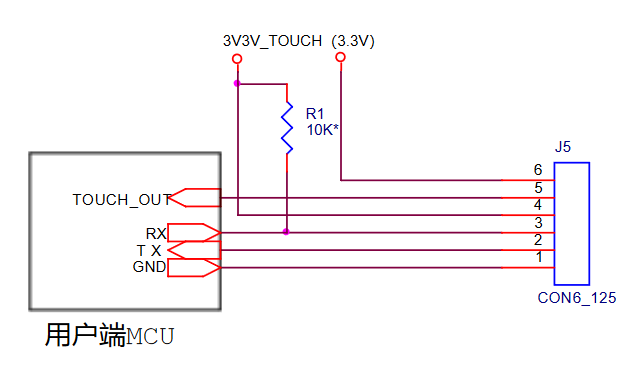
\includegraphics[scale=0.6]{imgs/FPM383C串口设备图.png}
    \caption{FPM383C串口设备图}    \label{FPM383C串口设备图}
\end{figure}


\subsubsection{通信模块选型}

    基于一般企事业单位对于考勤签到需求的需求,我计划提供多种不同的通信模块实现方便选用单位进行选择,
    其中传统基于 CH340 串口转 TTL 通信模块实现的简单串口通信主要适用于仅对于一两台设备进行支持的情况,
    而基于网卡模块间接通过网络方式拓展下位机数量的方式是主要计划实现的支持。
    针对于不同的预算管理需求,计划采用两种不同的方式实现网卡驱动,
    一种是基于 raspberry4B 板载 bcm54213PE 网卡芯片的驱动,
    另一种是基于 ENC28J60,一种基于 SPI 连接的外置 10BASE-T 以太网连接模块实现的。
    但是目前只实现了基于 BCM54213PE 网卡芯片驱动的支持。

    考虑到企事业单位对考勤签到的通用需求,我计划提供多种通信模块以便选用单位进行选择。
    一方面提供传统的 CH340 串口转 TTL 通信模块以适用于支持一到两台设备的简单串口通信。
    另一方面,我主要计划通过网络方式发送数据包以扩展下位机的数量。

    根据不同的预算管理需求,我计划采用两种方式来实现裸机网络通信支持。
    一种方式是实现 Raspberry Pi 4B 的板载 BCM54213PE PHY 芯片驱动;
    另一种方式则是采用E NC28J60 ,这一种基于 SPI 连接的外置 10BASE-T 以太网模块。

\subsection{硬件设计}

    由于本实现相对来说比较轻量化,不太需要外部模块的支持\ref{外部模块接线图},因此只通过杜邦线进行连接即可。

    \begin{figure}[ht]
    \centering
    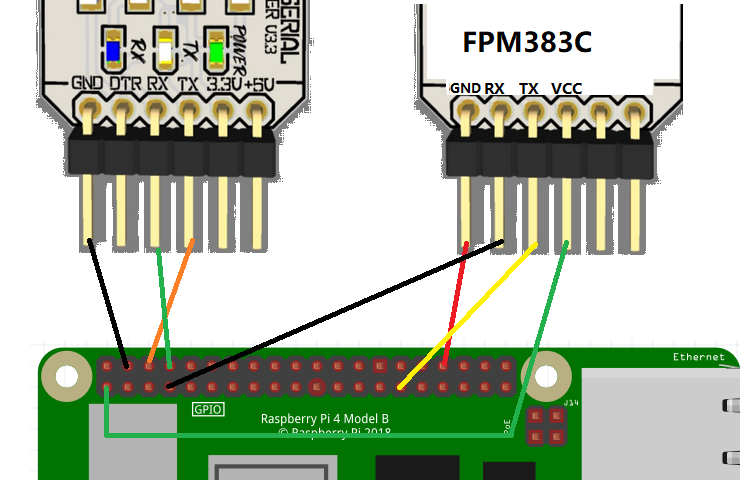
\includegraphics[scale=0.6]{imgs/接线图.png}
    \caption{外部模块接线说明图}    \label{外部模块接线图}
    \end{figure}

    \begin{itemize}
        \item 信号回返模块:
            按照最初的是采用额外的信号提示模块,基于树莓派 GPIO 电信号控制实现例如蜂鸣声或者 LED 闪烁提示当前已经完成
            打卡,但是这部分最后通过 FPM383C 模块内部的 LED 控制信号完成了提示操作,不再按照原先设想采用额外的无源蜂鸣
            器或者基于三极管实现的长延时信号灯。
        \item 指纹采集模块:
            本模块直接采用了现有的 FPM383C 指纹信号采集模块,直接通过调用树莓派串口服务,在原先串口通信模块的基础上实现
            对于指纹采集模块的通信。
            在硬件层面上,直接采用端子线将树莓派与 FPM383C 模块连接,连接示意图如\ref{外部模块接线图}右侧所示\cite{fpm383c-module-specification}。
        \item 网络通信模块:
            本模块主要使用了现有的树莓派板载 PHY 芯片 BCM54213PE 实现了对应 PHY 层信号解析,底层通过 RJ45 水晶头以
            双绞线直接连接笔记本网口。计划中额外支持 ENC28J60 模块还需要额外通过 GPIO 7,8,9,10,11,16,19,20,21 Pins 实现 SPI 端口连接
            来实现类似于树莓派板载 PHY 芯片的效果。
        \item 串口通信模块:
            在本次嵌入式实现中直接采用现成的 TTL 转 USB 模块 CH340 实现对于树莓派串口通信读取,具体接线方式如 \ref{外部模块接线图} 左侧所示,
            具体实现上通过被装载在树莓派上的系统中所默认打开的 UART0 串口(Pins 14,15)实现基本的信息传输
            \footnote{在后文中有指出,目前出于调试方便的目的,
            通过 rust 编译的裸机二进制文件会在树莓派上电发送信号(由SD卡上装载的默认内核实现)与前台 minipush 同步之后,
            经由串口被装载到设备内存中,最后默认内核会转交控制权给 ArceOS 的起始地址}
    \end{itemize}

\subsection{软件设计}

    由于本研究所采用的嵌入式应用场景相对单一,且仅涉及单应用程序单地址空间,
    % 由于本研究所采用的基础嵌入式应用程序所面对的的嵌入式应用场景相对较为单一,同时也是单应用程序单地址空间的。
    \footnote{虽然底层操作系统支持使用页表进行隔离,但是在应用层面上并没有使用到虚拟页表,只是在boot的时候使用了内核页表}
    因此整体软件设计相对较为简单,主要实现难度在驱动设计层面体现,具体内容与开发过程在第三章中进行呈现。
    在嵌入式应用中,系统通过循环读取UART串口设备的数据反馈,并通过ArceOS封装的底层以太网驱动,
    将分析后的结果根据需求封装成 UDP 包\footnote{保存打卡信息等},通过 RJ-45 接口发送至上位机的管理应用程序

    在上位机中通过简易的 python 客户端程序,对于嵌入式设备中传输的 UDP 包进行分析,实现基于 SQLite 数据库的简单指纹信息 CRUD,打卡数据 CRUD,
    与一个基于命令行实现的打卡记录查询与导出应用程序。

    \subsubsection{嵌入式软件设计}

    参照一般嵌入式考勤打卡设备的标准结构,我设计的嵌入式应用在完成对应变量初始化之后维持在一个主循环(如图\ref{algorithm::fingerprint_network_comm}中运行。
    一次循环包括收网络包\footnote{匹配帧头后向指纹模块下发对应UART包实现下载,删除指纹特征的效果}
    ,执行指纹匹配命令,对于指纹匹配结果进行查询,并在完成匹配时通过网络向上位机以特定的帧形式发送网络包告知其
    已经收到用户的打卡信息。

    \begin{algorithm}[htb]
        \caption{嵌入式设备主循环}
        \label{algorithm::fingerprint_network_comm}
        \begin{algorithmic}[1]
        \While{true} \Comment{嵌入式设备主循环事件}
            % \State \textbf{try} \Call{ReceiveData}{$socket, \& buf$}
            \If{\Call{Receive}{$socket, \& buf$} = Ok$(size, addr)$} \Comment{收到了网络包}
                \If{收包结果与特定帧头匹配}
                    \State 将对应 UART 帧转发给从属指纹识别模块
                \EndIf
                \State $buf \gets [0; 1024]$ \Comment{重置缓冲区}
                \State \Call{LogDebug}{\textbf{error}} \Comment{打印其他错误}
            \EndIf
        
            \State \Call{Write}{serial, \text{search\_fingerprint\_match\_pattern}} \Comment{向设备发送匹配命令}

            \State \Call{Delay}{10} \Comment{等待模块进行指纹匹配}
            \State \Call{GetFrame}{$serial$} \Comment{处理返回帧}
            
            \State \Call{Write}{serial, \text{check\_match\_\_result\_pattern}} \Comment{向设备发送匹配命令}
        
            \If{$frame \gets$ \Call{GetFrame}{$serial$}}  \Comment{对于返回包进行分析}
                \State \Call{Assert}{$frame$, CmdType::CheckMatchFingerprint} \Comment{确保应答包一致}
                
                \If{\Call{Any}{$data, \neq 0$}}
                    \State \textbf{initialize} $sign\_in\_buf \gets [0x46, 0x69, \ldots, 0x20]$ \Comment{网络包}
                    \State \Call{SetSignInData}{$frame, sign\_in\_buf$} \Comment{根据应答包设置 buf 中与ID部分}
                    \State \Call{SendTo}{$local\_socket, sign\_in\_buf, target\_socket$}
                    \State \Call{Write}{serial, \text{green\_flashing\_pattern}} \Comment{向设备发送绿灯闪烁}
                \EndIf
                \State \Call{GetFrame}{$serial$}
            \EndIf
        \EndWhile
        \end{algorithmic}
        \end{algorithm}
        

    \subsubsection{数据库设计}

    由于对应本次嵌入式设计的上位机中的操作需求相对较为简单直白。同时,不同于课堂考勤系统等需要额外的提供很多
    诸如教学班,教室,教师等信息的需求,需要维持一系列诸如教学班表,教师表,学生表等。\cite{基于WiFi探针的智能考勤系统设计}
    本次嵌入式软件在功能层面仅需要完成简单的考勤打卡记录,指纹特征模块的存储
    的功能,因此在表实现上仅需要维持三个表的存在,分别是指纹特征表,员工信息表,考勤打卡表。

    因此,在这样的一个简单的的嵌入式项目中使用诸如 Oracle, MySQL, PostgreSQL 等大型企业级数据库是没有效率
    的行为。在设计中综合考量了一系列如 SQLite, LMDB 等嵌入式常用的数据库,考虑到常用性,库支持程度等因素之后
    选用了 SQLite 作为嵌入式信息存储的数据库。

    \begin{description}
        \item[用户信息表] 存储常见的用户信息数据

            在用户信息表\ref{tab:userInfo}中完成对于用户ID,指纹特征信息的存储属于一种最基本的考勤系统嵌入式设计需求。在本表中我将 user\_id 作为主键,唯一性的声明用户的身份,并且将其与唯一对应的指纹信息进行关联,在还引入了指纹特征表的主键 finger\_print\_id 实现级联删除。

            同时,考量到在实际上位机将对应数据下载到嵌入式设备的从属指纹识别模块的时候需要先向
            其发送一个 指纹特征信息下载 包,在该包中声明本次传输的信息会被装载到哪个指纹特征ID以及传输的指纹特征数据长度,以方便指纹模块根据长度截断数据。在本表中还专门提供了与
            finger\_print\_id 对应的长度数据。

            \begin{lstlisting}[language=SQL
                , caption={用户信息表}
                , label = {tab:userInfo}
                , breaklines=true
                , breakatwhitespace=true]
CREATE TABLE IF NOT EXISTS user (
    user_id INTEGER PRIMARY KEY AUTOINCREMENT,
    user_name TEXT NOT NULL,
    finger_print_id INTEGER,
    finger_print_len INTEGER,
    other_message TEXT,
    FOREIGN KEY (finger_print_id) REFERENCES fingerPrint(finger_print_id)
);
            \end{lstlisting}

        \item[指纹特征表] 存储指纹 ID,指纹特征长度,指纹特征信息等内容。
        
            在数据传输过程中,每一次传输除最后一包外,均只发送128位的指纹特征数据。这要求在上位机中首先组合完整的指纹特征信息,然后再将其存储到SQLite数据库中。这种处理方式不仅增加了上位机的资源消耗(在SQLite中,数据以页面形式存储),还需要在数据下载到嵌入式设备的指纹识别模块前进行再次切分,显著增加了工作量。因此,我们选择不使用指纹ID作为主键,而是直接在上位机接收到的数据中,根据每个数据包自带的frame号对数据进行简单分割,以简化处理过程。
        
            在指纹特征表\ref{tab:fingerprintInfo}中存储了对应于指纹ID的 frame 号\footnote{用于标识数据帧},二进制指纹特征信息信息。
            在本系统重我们没有选择使用指纹 ID 作为主键,主要是考量到在实际进行发送的时候由于指纹模块通信协议要求采用的是分段发送数据的策略,\ref{fpm383c-modular-communication-protocol}
            即除去传输的最后一个包,每次向指纹模块传输数据的时候,最高只能在一个帧中放置 128 字节的指纹特征数据。
            在这种情况下先在上位机中对于对应指纹特征信息进行组合,再存储到 SQLite 中,不仅会导致对于上位机更高的资源占用\footnote{在SQLite中以页的信息存储对应数据},
            在实际将特征数据下载到嵌入式设备的从属指纹识别模块的时候同样需要进行切分之后再发送,
            无疑是增添了许多无异议的工作量,因此最终并没有采用这种形式存储指纹特征数据。
            而是根据对应对应二进制数据由指纹模块上传到上位机中自带有的 frame 号 对逐帧的数据进行简单的分割。

            \begin{lstlisting}[language=SQL
                , caption={指纹特征表}
                , label = {tab:fingerprintInfo}
                , breaklines=true
                , breakatwhitespace=true]
CREATE TABLE IF NOT EXISTS fingerPrint (
    id INTEGER,
    frame INTEGER,
    data BLOB NOT NULL,
);
            \end{lstlisting}          


        \item[考勤打卡表] 记录考勤打卡的时间信息
        
            在考勤打卡表\ref{tab:signIn}中主要保存对应于 user\_id 的打卡数据,其中通过默认CURRENT
            \_TIMESTAMP的方式自动插入了对应的时间戳数据,方便用户进行插入操作。

            \begin{lstlisting}[language=SQL
                , caption={考勤打卡表}
                , label = {tab:signIn}
                , breaklines=true
                , breakatwhitespace=true]
CREATE TABLE IF NOT EXISTS signIn (
    user_id INTEGER,
    time TEXT DEFAULT CURRENT_TIMESTAMP
)
            \end{lstlisting}    

    \end{description}

    \subsubsection{功能说明}

    \begin{description}
        \item[指纹注册] 由上位机中自动完成指纹注册,通过上传命令,获取对应ID的指纹特征信息并以UDP包的形式下发到下位机中的指纹模块。
        
        指纹注册功能主要在上位机中完成,这主要是考量到在 HR 处实现人事登记等操作
        更加合乎一般企业的考勤流程。
        
        通过 0x0118 命令\ref{uart::auto-register},实现自动注册功能,该命令会自动完成采图、提取、拼接、保存等操作,
        该部分通过分析返回包中的ID和注册进度进行操作,在注册进度达到 0x64 时终止注册流程。

        \begin{table}[htbp]
            \resizebox{\textwidth}{!}{%
                \begin{tabular}{|l|l|l|l|l|l|l|l|}
                \hline
                \multicolumn{1}{|c|}{校验密码} & CMD类型 & CMD号 & 等待手指 & 按压次数 & ID\_H & ID\_L & 校验和  \\ \hline
                0x00 0x00 0x00 0x00        & 0x01  & 0x18 & 0x01 & 0x06 & 0xFF  & 0xFF  & 0xE2 \\ \hline
                \end{tabular}
            }
            \caption{自动注册命令用户层帧} \label{uart::auto-register}
        \end{table}

        在注册完成之后,通过上载命令\ref{uart::upload-info},向指纹模块获取特定 ID 号的指纹特征信息长度,
        然后再通过 \ref{uart::upload-data} 命令,从指纹模块获取对应分片的指纹特征信息。
        在将信息存储到数据库的同时,还通过 UDP 包的形式,将对应的数据发送到树莓派,树莓派再将对应指纹特征信息
        下载到树莓派对应的指纹模块上,由此完成了一次标准的指纹注册功能。

        \begin{table}[htbp]
            \resizebox{\textwidth}{!}{%
                \begin{tabular}{|l|l|l|l|l|l|}
                \hline
                \multicolumn{1}{|c|}{校验密码} & CMD类型 & CMD号 & ID\_H & ID\_L & 校验和  \\ \hline
                0x00 0x00 0x00 0x00        & 0x01  & 0x53 & 0x00  & 0x01  & 0xAB \\ \hline
                \end{tabular}
            } \caption{获取上传信息命令用户层帧} \label{uart::upload-info}
        \end{table}

        \begin{table}[htbp]
            \resizebox{\textwidth}{!}{%
            \begin{tabular}{|l|l|l|l|l|l|l|l|}
                \hline
                \multicolumn{1}{|c|}{校验密码} & CMD类型 & CMD号 & ID\_H & ID\_L & NUM\_H & NUM\_L & 校验和  \\ \hline
                0x00 0x00 0x00 0x00        & 0x01  & 0x51 & 0xFF  & 0xFF  & 0x00   & 0x00   & 0xAC \\ \hline
                \end{tabular}
            } \caption{获取指纹特征命令用户层帧} \label{uart::upload-data}
        \end{table}

        \item[指纹删除] 在上位机中完成指纹删除操作,通过下行 Udp 包,删除指纹模块中对应 ID 的指纹特征信息。
        
        指纹删除功能主要在上位机中完成,在出现指纹出现问题的时候,由 HR 执行运行函数,自动化删除数据库中员工对应的指纹特征编号,
        同时将删除指纹特征编号的命令通过下面的指令\ref{指纹特征清除}经由树莓派下发到指纹终端,根据不同的需求,在下面的帧中配置不同的格式。

        \begin{table}[ht]
            \resizebox{\textwidth}{!}{%
                \begin{tabular}{|l|l|l|l|l|l|l|}
                \hline
                \multicolumn{1}{|c|}{校验密码} & CMD类型 & CMD号 & CL\_FLAG & ID\_H & ID\_L & 校验和  \\ \hline
                0x00 0x00 0x00 0x00        & 0x01  & 0x51 & 03       & 0xFF  & 0xFF  & 0xAC \\ \hline
                \end{tabular} 
            } \caption{指纹特征清除} \label{指纹特征清除}
        \end{table}

        \item[指纹考勤登记] 在下位机从属指纹模块中完成基于指纹的考勤实现。
        
        下位机会循环的向指纹模块询问指纹能否匹配\ref{询问是否匹配},并按照匹配应答包\ref{匹配应答包}格式返回对应结果,
        根据对应的匹配分数以及是否完成匹配。

        当当前指纹被实际判断匹配成功,对应的数据就会被放在下面的帧结构中,再通过 UdpSocket 发送到上位机的 Socket,
        上位机中利用 Python Socket 对于 5555 端口进行长期监听,对所有监听到的数据包进行匹配,当前后帧结构一致的情况下
        将其中包含的 ID 按照 sqlite 的规定插入到对应表中
        \footnote{sqlite中有一种名为 CURRENT\_TIMESTAMP 的默认属性,会默认将插入项的时间作为一个元素一起插入}。

        \begin{table}[ht]
            \resizebox{\textwidth}{!}{%
                \begin{tabular}{|l|l|l|l|}
                \hline
                \multicolumn{1}{|c|}{校验密码} & CMD类型 & CMD号    & 校验和  \\ \hline
                0x00 0x00 0x00 0x00        & 0x01  & 0x21 / 0x22 & 0xAC \\ \hline
                \end{tabular}
            }  \caption{询问是否匹配,查询匹配结果} \label{询问是否匹配}
        \end{table}

        \begin{table}[htbp]
            \resizebox{\textwidth}{!}{%
                \begin{tabular}{|l|l|l|l|l|l|l|l|}
                \hline
                \multicolumn{1}{|c|}{校验密码} & CMD类型 & CMD号 & 错误码                 & 匹配结果      & 匹配分数      & 匹配ID      & 校验和  \\ \hline
                0 0 0 0        & 0x01  & 0x51 & 0 0 0 0 & 0x00 0x01 & 0x27 0x0F & 0x00 0x03 & 0xAC \\ \hline
                \end{tabular} 
            }  \caption{匹配应答包格式} \label{匹配应答包}
        \end{table}

        \item[考勤记录读取] 根据一般企事业单位的考勤系统的历史发展来看,读取员工考勤记录属于考勤系统的必备功能。
        
        本功能主要实现在上位机处,由上位机调用函数对于原先保存在 SQLite 中的考勤打卡表与员工-指纹特征对应表进行自动关联,并且
        基于一定的逻辑分析打印出员工的详细打卡数据与月度打卡数据。
        \newpage
    \end{description}
      

